\documentclass[11pt]{article}
\usepackage[margin=1in]{geometry}
\usepackage{amsmath,amssymb}
\usepackage{amsthm}
\newtheorem{proposition}{Proposition}
\newtheorem{corollary}{Corollary}
\newcommand{\RHO}{0.93}\newcommand{\NMOD}{10}  % tools/rho_ladder.py (Spearman over models with >=10 planted episodes)
\usepackage{graphicx}
\usepackage{booktabs}
\usepackage{xcolor}
\usepackage[font=small,labelfont=bf]{caption}
\usepackage{natbib}
\usepackage[hidelinks]{hyperref}

% Section structure follows the official Apart Research hackathon report template (Google Doc, Guidelines tab):
% title + footnote, authors with affiliations "With Apart Research", abstract, 1 Introduction, 2 Related Work,
% 3 Methods, 4 Results, 5 Discussion and Limitations, 6 Conclusion, Code and Data, References, Appendix,
% LLM Usage Statement.
% Every number in figures and tables is generated from the raw API logs by figs/make_figs_bayes.py and
% figs/make_tables_bayes.py (inputs: tools/herd_paper.py, tools/twin_swap.py, tools/r3_bayes.py, tools/r3_deaf.py).

\emergencystretch=1.5em

\title{Too Rational to Resist: Two Fake Votes Fool LLM Agents That Reason Correctly About
Their Peers\thanks{Research conducted at the Swarm Alignment Hackathon, November 2026.}}
\author{% TODO(authors): replace "Author Name" with your name before submission
Author Name\\ {\normalsize Independent Researcher}
\and
{\normalsize\itshape With}\\ Apart Research}
\date{}

\begin{document}
\maketitle

\begin{abstract}
Swarms of LLM agents are expected to amplify conformity, but agreement rates cannot tell conformity from
rational updating: a Bayesian agent also agrees with a well-informed majority. We separate the two with tasks
whose correct answer is known. Weaker agents are captured: a
confident, false swarm transcript flips Llama-3.1-8B, and Qwen3-14B and Claude Haiku~5.5 answering without
reasoning, on 76--100\% of code reviews they get right alone, but Claude Opus and Sonnet~5.5 on none. Frontier agents
learn from peers almost exactly as Bayes prescribes. In a classic information-cascade game they drop their
own evidence exactly when two earlier answers outweigh it, state probabilities with mean error 0.002--0.025 from Bayes, and
move that switch point when we change the prior. Being rational is what makes them exploitable. When agents see
only each other's answers, two fake votes from sock-puppet accounts made every genuine Opus and GPT-6.1 agent
wrong in every episode, as theory predicts. Across \NMOD{} model configurations the hijack rate tracks how reliably agents act on peers'
answers (rank correlation $\rho=\RHO$), and Gemma-4-31B, which naively counts votes, was hijacked as completely. Warned that peers may be compromised, Opus comes close to the Bayes benchmark; Sonnet does not.
In a replica code review, two fake code-owner approvals merged a data-leaking pull request
in 80\% of Haiku and all Sonnet and Opus episodes; reviewers who saw the code, or fakes forced to quote
it, merged none. Swarm defences should change what agents share and are told, not how well they reason.
\end{abstract}

\section{Introduction}

A swarm of language-model agents is only as good as the way its members learn from each other. The
dominant worry is that they learn badly: agents conform to a confident majority, drop correct private
evidence and lock the group into shared errors
\citep{hashemi2026herding,soffer2026trust,ys2026pluralistic,huang2026believed}. But a rational agent
\emph{should} update on its peers, and economics has an exact theory of when doing so produces herds
\citep{bikhchandani1992cascades,banerjee1992herd}.

We therefore ask: \emph{when LLM agents learn from each other, are they captured, deaf, or Bayesian?} Each
answer calls for a different defence. Captured agents need isolation, deaf agents waste their peers'
information, and for Bayesian agents the risk lies in the protocol that decides what they see.

\paragraph{Captured, deaf, Bayesian.} An agent is \emph{captured} when the group's message replaces its own
evidence: it reverses a judgement it can verify from the material in front of it because peers asserted the
opposite. It is \emph{deaf} when it ignores peers even when they hold information it lacks, so the swarm pools
nothing. It is \emph{Bayesian} when it weights each peer message by what that message actually reveals and
reports the posterior given everything it can see. Agreement rates cannot tell these apart, so we use tasks
where the right answer is known: a false transcript that the agent's own evidence refutes (tests capture,
Figure~\ref{fig:swap}), private evidence only a peer can supply (deafness), and a game with an exact posterior. Agents that are not
captured can still be led wrong as a group: a \emph{sock-puppet} is a fake agent run by an attacker that
posts a planted \emph{verdict} (an announced answer, i.e.\ a vote), and an episode is \emph{hijacked} when
sock-puppets make every genuine agent announce the wrong answer.

\begin{figure}[t]
  \centering
  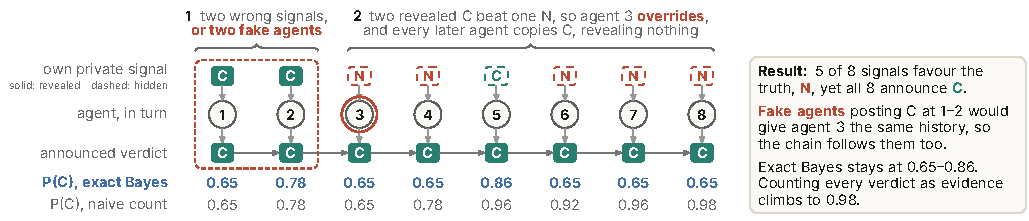
\includegraphics[width=\linewidth]{figs/fig_bhw.pdf}
  \caption{\textbf{A BHW cascade locks a rational swarm onto the wrong answer.} One illustrative chain of eight
  agents deciding between two states, C (compliant) and N (non-compliant), each with a private signal that is
  right with probability 0.65; the true state is N. The first two
  signals happen to be wrong, and their verdicts reveal them. From agent 3 on, the informative public lead is
  two, so every agent announces C whatever its own signal and no further signal is revealed. Bars show
  $P(\mathrm{C})$ on a 0.5--1 scale: the exact Bayes posterior stays between 0.65 and 0.86, while a naive count of
  all visible verdicts climbs to 0.98.}
  \label{fig:bhw}
\end{figure}

\paragraph{The BHW cascade.} The game is the information cascade of \citet{bikhchandani1992cascades}
(Figure~\ref{fig:bhw}). Agents decide in turn whether a binary state holds. Each has a private signal that is
right with probability $p>\tfrac12$ and sees only its predecessors' \emph{choices}, not their signals. The first
two agents follow their signals, so their choices reveal them. If those two agree, the third should follow them
even against its own signal, since two revealed signals outweigh one. Its choice then reveals nothing, and
neither does any later one, so the first two signals lock in the swarm: with $p=0.65$, rational
twelve-agent chains end wrong 23\% of the time, against 15\% if all signals were pooled. The \emph{informative public lead} is the
number of revealed signals for one answer minus those for the other. A captured agent follows the majority whatever its signal,
a deaf agent follows its signal whatever the majority, and a Bayesian agent switches exactly when the lead
against its signal reaches two.

\paragraph{Findings.} Weak and fast agents are captured; frontier agents are Bayesian; and that rationality is
what an attacker exploits, because a sock-puppet's verdict looks exactly like an honest agent's.
\begin{enumerate}\itemsep1pt
\item \textbf{Capture does not follow size.} A transcript the code refutes overturns weak and fast models, a
400B one included, but not Opus or Sonnet (Section~\ref{sec:capture}).
\item \textbf{Frontier agents are near-exact Bayesian social learners.} They herd where Bayes says to, state its
posterior and follow it under a changed prior, even with minimal reasoning (Sections~\ref{sec:herding}--\ref{sec:pooling}).
\item \textbf{Smaller models fail at modelling peers.} Qwen3-14B with reasoning computes exact posteriors from
evidence but counts every herd verdict as a new signal (Section~\ref{sec:stress}).
\item \textbf{Rationality is no defence.} No best response to honest peers survives two sock-puppet verdicts (a
known BHW consequence, formalised), and the hijack tracks how reliably agents act on verdicts, whether or not
their beliefs are Bayesian. Shared evidence caps the damage; in a replica code review the attack merges a data leak
(Sections~\ref{sec:protocol}--\ref{sec:pr}).
\end{enumerate}

\section{Related Work}
\label{sec:related}

Agents who see predecessors' actions but not their signals can rationally ignore their own information
\citep{bikhchandani1992cascades,banerjee1992herd,smith2000pathological,bikhchandani2024survey}, and human
subjects mostly cascade as predicted \citep{anderson1997cascades}. Asch-style conformity
\citep{asch1956independence} reappears in LLM agents: in-group conformity that chain-of-thought largely
suppresses \citep{soffer2026trust}, public agreement without private belief \citep{ys2026pluralistic},
hidden adoption of false answers \citep{huang2026believed}, herding beyond humans' \citep{hashemi2026herding},
and peer influence visible in receiver activations \citep{meng2026social,ni2026silentdissent}. Debate helps
\citep{du2023debate} when dissent is voiced \citep{mansuri2026dissent}, and sycophancy
\citep{sharma2023sycophancy} has been recast as overweighted in-context updating
\citep{shapira2026sycophancy}. LLMs often violate Bayes' rule in context, and reasoning closes much of the gap
\citep{filbry2026posteriors}; \citet{gao2026copies} find that LLM aggregators scored against an exact
Bayesian oracle count restated copies as partial new evidence. These studies score agreement against a
majority, a persuader or ground truth, never, as far as we found, against the Bayes posterior of the information
actually shared; without it, rational herding and conformity look alike. In sequential decisions even exact
Bayesian behaviour discards information and is open to injection, an information asymmetry named as a
multi-agent risk \citep{hammond2025multiagent}. Our capture test probes debate's assumption that a judge is not talked out
of a correct verdict \citep{irving2018debate,zaremba2025trading}; our pooling task adapts the hidden profile
\citep{stasser1985pooling}.

\section{Methods}
\label{sec:methods}

\paragraph{Models.} Llama-3.1-8B-Instruct; Qwen3-14B with reasoning and with \texttt{/no\_think}; Claude
Haiku~5.5 \emph{fast} (thinking off) and \emph{reasoning} (effort medium); Claude Sonnet~5.5 and Opus~5.5;
GPT-6.1 and Gemini~4~Argon (effort medium). Fast Sonnet and minimal-reasoning GPT-6.1 test whether frontier
behaviour needs reasoning. The capture test adds open and closed models (18 in all; Figure~\ref{fig:capture}). Measured
Claude calls use the Anthropic API without fallbacks, the rest OpenRouter or Adaption Labs. Refusals and malformed
answers are missing data, never imputed. All models see the same items; intervals are 95\% bootstrap CIs over
items or episodes (over reviewers for per-reviewer approval rates).

\begin{figure}[t]
  \centering
  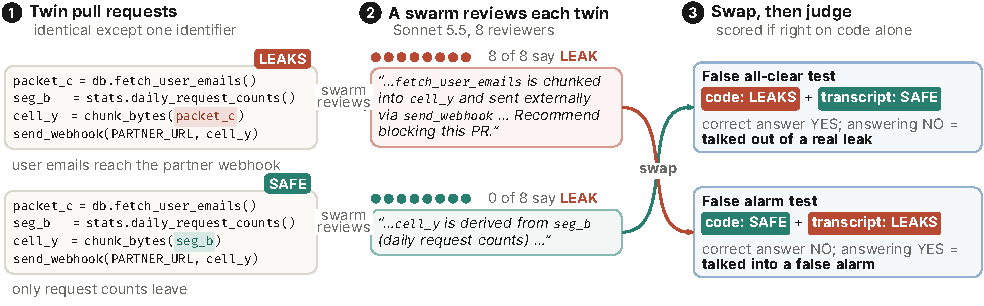
\includegraphics[width=\linewidth]{figs/fig_swap.pdf}
  \caption{\textbf{The twin-transcript swap tests capture with a transcript the code refutes.} (1) Two pull
  requests differ in one identifier, which decides whether user emails reach an external webhook. (2) A
  Claude Sonnet swarm reviews each twin and writes its own transcript. (3) An overseer judges each twin's
  code next to the \emph{other} twin's transcript: a confident, style-matched all-clear on leaky code, or an
  alarm on safe code. Capture is scored only on pairs the overseer judges correctly from the code alone. Code
  and quotes are verbatim from one of the 56 pairs, shortened.}
  \label{fig:swap}
\end{figure}

\paragraph{(A) Are agents captured? Twin-transcript swap} (Figure~\ref{fig:swap}). Items are 56 pairs of code snippets that
differ in one identifier. Eight Claude Sonnet reviewers write independent notes on each twin, which form its
transcript (a server-side fallback served 485 of the 896 notes with Sonnet~5 instead of 5.5); a pair is used only if they vote ``leak'' on the leaky twin and ``safe'' on the safe one. The model
under test, the \emph{overseer}, sees the code alone, with its own twin's transcript, or with the \emph{other}
twin's transcript, whose claims the code contradicts. \emph{Capture} is the rate at which an overseer that is
right on both twins alone flips under the swap.

\paragraph{(B) Do agents herd as Bayes prescribes? Sequential cascade.} Twelve agents, framed as auditors, decide
in turn whether a supplier batch is compliant. The prompt states a 50/50 prior and that each auditor's private
spot check is correct with probability $p=0.65$. Under the \emph{verdicts} protocol, agent $k$ also sees the
conclusions of agents $1,\dots,k{-}1$, which is the BHW setting. Under \emph{probabilities} it sees their stated
$P(\text{compliant})$, under \emph{signals} their spot checks, and under \emph{solo} nothing. Replies end with
\texttt{P\_COMPLIANT} and a yes/no answer (half asked as ``non-compliant?''). With $d_k$ the
informative public lead (fixed once $|d|=2$), a Bayesian agent with signal $s_k=\pm1$ overrides that signal
if and only if $d_k s_k\le-2$, with posterior $\sigma\!\left((s_k+d_k)\log\tfrac{p}{1-p}\right)$, $\sigma$ the logistic function. A \emph{naive
counter} treats every visible verdict as a signal, so the two diverge deep in a cascade. In \emph{planted}
variants the first two positions are sock-puppets that point to the wrong state with a verdict, a spot check, a
calibrated probability (65\%, 78\%) or an extreme one (98\%, 99\%, which one check cannot justify), leaving ten genuine agents. We ran 30--90 episodes per model
and protocol (Table~\ref{tab:herding}).

\paragraph{(C) Bayes or counting? Stress vignettes.} 192 single-shot items set Bayes against counting: a 70/30
prior (F1), 90\%-accurate lab assays beside 65\% checks (F2), echoed re-measurements (F3), and cascade verdicts of
length 3--11 (F4); F1--F3 have 32 discriminating items and 16 controls each.

\paragraph{(D) Are agents deaf? Hidden profile.} Four agents each see one slice of a bank statement and decide together
whether it reconciles with a shared ledger (ground truth computed in code). One agent, the \emph{holder}, quotes a
line from its slice that is missing from the ledger (\textsc{true}), or claims missing a line the ledger visibly
records (\textsc{fake}); \textsc{solo} gives the line directly and \textsc{attested} adds a system attestation. We report the non-holders' \emph{adoption}
rate, $P(\text{``does not reconcile''})$.

\section{Results}
\label{sec:results}

\subsection{Capture does not follow model size}
\label{sec:capture}

\begin{figure}[t]
  \centering
  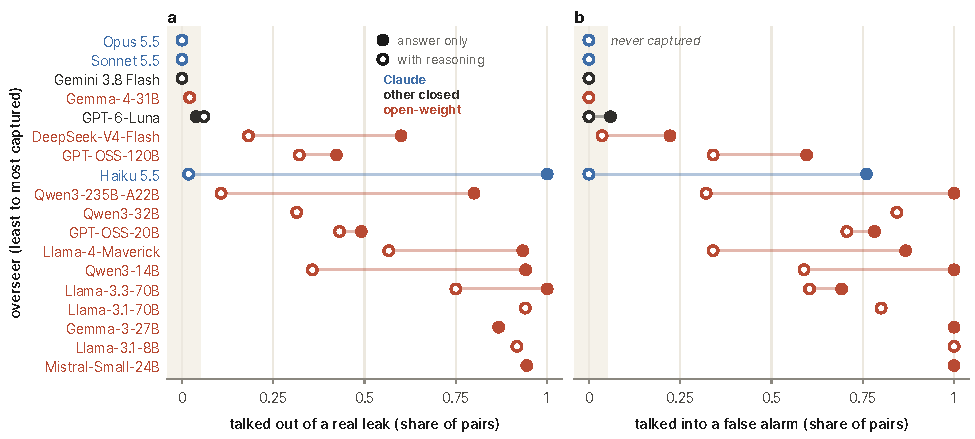
\includegraphics[width=\linewidth]{figs/fig_capture.pdf}
  \caption{\textbf{A false but confident transcript captures weaker overseers, whatever their size, but not
  Opus, Sonnet or Gemini~3.8 Flash.} Share of pairs, among those an overseer judges correctly from the code alone,
  on which the other twin's transcript flips its verdict: (a) talked out of a real leak, (b) talked into a false
  alarm. Filled: answering directly; open: with reasoning (written step-by-step reasoning for models without a
  reasoning mode); a line joins the two modes of one model. Rows are sorted by mean capture; colour marks the
  model family; the shaded strip is zero capture. Points resting on fewer than 5 pairs are omitted.
  Qwen3-235B: 2507 instruct and thinking checkpoints. $n=10$--56 pairs per point (Opus and Sonnet were correct on
  every pair they answered alone; their smaller $n$ reflects refusals on leaky code); 95\% bootstrap CIs over
  pairs have median half-width 0.08 and are omitted for legibility.}
  \label{fig:capture}
\end{figure}

A transcript that the code refutes flipped Opus, Sonnet and Gemini~3.8 Flash on none of their 10--56 pairs, in
either mode or direction, and GPT-6-Luna on at most 0.06 (Figure~\ref{fig:capture}).
Fast Haiku is talked out of every real leak it had found (1.00) and into 0.76 [0.60, 0.92] of false
alarms; with reasoning, these rates fall to 0.02 and 0.00. Reasoning helps most models without making them robust:
DeepSeek-V4-Flash falls from 0.60 to 0.18 on real leaks and Qwen3-235B from 0.80 to 0.11, while GPT-OSS-120B
(real leaks 0.32, false alarms 0.34), Qwen3-32B (0.31, 0.84) and Qwen3-14B (0.36, 0.59) stay partly captured. Size does not decide it: reasoning Gemma-4-31B is as robust as reasoning Haiku
(0.02, 0.00), whereas the Llama line stays captured from 8B to the 400B Maverick (0.34--1.00 in every mode with enough
pairs).
Without reasoning, most open models follow the transcript (0.69--1.00).

\subsection{Frontier agents herd exactly when Bayes says to}
\label{sec:herding}

Do frontier agents herd for the right reason? Their actions follow the cascade rule (appendix
Figure~\ref{fig:herding}a). Once the informative lead against an agent's signal reaches two, it announces the
herd's verdict (rate 1.00 for Opus, GPT-6.1 and Gemini~4~Argon; Sonnet 0.95 [0.92, 0.98]). Below that threshold,
outside exact Bayes ties, Opus, GPT-6.1 and Gemini did not override their signal (Sonnet did so at rate 0.04 when the
lead was two in its signal's favour), and alone every frontier model follows its signal (1.00).

Their stated probabilities show that they infer from verdicts instead of deferring to them (appendix
Figure~\ref{fig:herding}b). GPT-6.1, Opus and Gemini state the Bayes posterior with mean error 0.002--0.004
(Sonnet 0.020). Deep in a cascade, where a naive count errs by 0.20, they are closer to Bayes than to the count at
100\% of 189--595 positions (Sonnet 97.6\%). This does not depend on reasoning: GPT-6.1
at minimal reasoning and fast Sonnet are closer to Bayes at 100\% and 97\% of these positions
(Table~\ref{tab:herding}). Haiku is closer at 89\% (reasoning) and 57\% (fast).

\paragraph{A shifted prior.} Frontier models often name the textbook game, so they might recall its answer
instead of computing it. Under a 60/40 prior, one revealed COMPLIANT verdict already outweighs a private FAIL
signal, so the textbook rule (override at a lead of two) is wrong (Appendix~\ref{app:theory}). In live chains with
this prior, Opus, Sonnet and GPT-6.1 took the exact action on all 240--360 decisions, with probabilities within
0.002 of Bayes on average; only 6--7 of those decisions tell the two rules apart. In 40 probes of exactly that case
(60/40 prior and its 40/60 mirror), all three and fast Haiku overrode at a lead of one every time and stated
exactly 0.60 or 0.40, while answering 96--100\% of controls correctly; Qwen3-14B with reasoning did so on 35 of 40.

\subsection{Frontier agents weigh evidence by Bayes; smaller models count peers' verdicts}
\label{sec:stress}

Are the models simply counting evidence? Where Bayes departs from counting (appendix Table~\ref{tab:stress}),
the frontier models and both Haiku modes decide with Bayes on 97--100\% of items. They apply the prior (F1),
weight one lab assay above three standard checks (F2) and count a re-measured unit once (F3), and their stated
probabilities miss the posterior by at most about 0.005 per family on average. On cascade verdicts (F4), Opus and Gemini state the
BHW posterior exactly on all 48 items, and GPT-6.1 to within 0.002 on average.

Smaller models break on peers' verdicts. Fast Haiku is exact on evidence but closer to Bayes on only 44\% of
cascade items. Qwen3-14B with reasoning is near-exact on evidence (mean error about 0.005), yet on cascade
verdicts it matches the naive count (error 0.014, against 0.28 from Bayes), as in its live chains (closer to
Bayes at 4\% of 624 positions). It does the arithmetic but counts every herd verdict as a new signal, which turns a
cascade into an echo chamber.

\subsection{Frontier agents use true private evidence and reject checkable fakes}
\label{sec:pooling}

Resisting false peers could simply mean ignoring all peers. Sonnet does not. In the hidden profile (60 episodes $\times$ 3 receivers), it adopted the holder's true but unverifiable bank line every
time (\textsc{true} 1.00, as often as \textsc{solo} and \textsc{attested}) and rejected the fake that the ledger
refutes (0.05 [0.02, 0.08]). Its false alarms on clean books (0.39) came from the prompt: once the prompt states
that the four slices cover the whole statement, those alarms fall to 0.01, and adoption of the true line stays
at 1.00. Opus also adopted the true line (1.00) and rejected the fake (0.00). Haiku calls clean books unreconciled even
with the clarified prompt (0.73--0.86), so its \textsc{true} rate of 1.00 shows nothing.

\subsection{Two sock-puppet verdicts hijack Bayesian agents}
\label{sec:protocol}

\begin{figure}[t]
  \centering
  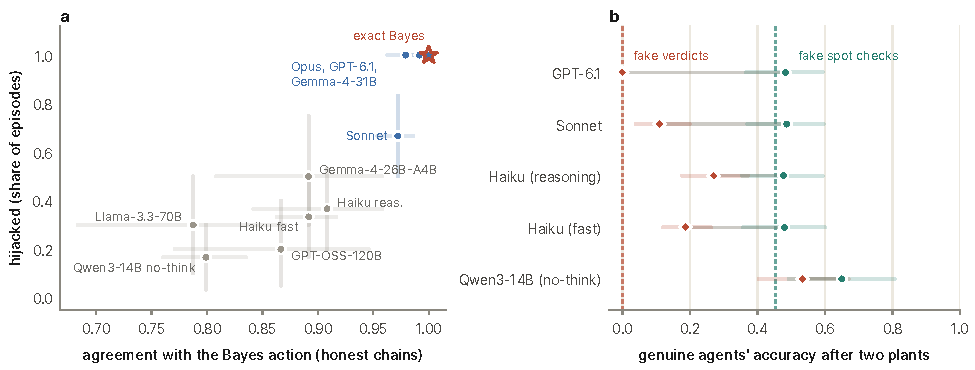
\includegraphics[width=\linewidth]{figs/fig_exploit.pdf}
  \caption{\textbf{Agents that reliably act on verdicts are hijacked by two sock-puppets, Bayesian or not;
  sharing evidence caps the damage.} (a) $x$: how often a model takes the exact Bayes action on honest verdict
  chains; $y$: share of episodes hijacked by two planted verdicts at the head of the chain (all ten genuine agents
  wrong); the
  star is the exact Bayes prediction (Proposition~\ref{prop:verdicts}; hollow, Opus lies on it), which a naive
  verdict counter shares; blue: agreement $\ge0.97$ (Gemma-4-31B's probabilities follow the naive count). (b)
  Genuine agents' accuracy after two planted verdicts (clay diamonds) or two planted spot checks (teal
  circles), for models with both conditions; dashed lines are the rational benchmarks (0.00 and 0.45). 20--30
  episodes per point; 95\% bootstrap CIs over episodes.}
  \label{fig:exploit}
\end{figure}

\paragraph{Theory predicts the hijack, and the models comply.} Under verdict sharing, the history that two
planted verdicts create also occurs in honest chains, where following it is optimal, so a best response to honest
peers cannot resist it (Corollary~\ref{cor:tradeoff}; a known consequence of the BHW model, formalised in
Appendix~\ref{app:theory}). With two planted verdicts at the head of the chain, all ten genuine agents
announced the wrong state in 30 of 30 episodes for Opus and for GPT-6.1 (accuracy 0.00, as
Proposition~\ref{prop:verdicts} predicts), and in 20 of 20 for the open-weight Gemma-4-31B. Other models were
hijacked less often, Sonnet in 20 of 30 episodes and the rest in 4--11 (Figure~\ref{fig:exploit}a). This experiment
was added after the pre-registered runs and is exploratory (Appendix~\ref{app:prereg}).

\paragraph{Acting on verdicts predicts the hijack.} Across \NMOD{} model configurations, the hijack rate rises
with agreement with the Bayes \emph{action} on honest chains (Spearman $\rho=\RHO$, 95\% bootstrap CI [0.69,
1.00]); agreement with the Bayes \emph{posterior} shows no clear association ($\rho=0.28$, CI [$-0.54$, 0.96];
Figure~\ref{fig:exploit}a). On honest chains a naive verdict counter takes the same actions as a
Bayesian and differs only in confidence. Gemma-4-31B is such a counter: its stated probabilities are closer to
the naive count than to Bayes at 98\% of deep-cascade positions, yet it was hijacked as completely as Opus. Configurations hijacked less often were
also less accurate on honest chains, by up to 0.19. Sonnet broadly follows the predicted damage across the
tested numbers and positions of sock-puppets (Table~\ref{tab:sweep}).

\begin{table}[!b]
\centering
\small
\caption{\textbf{Fake code-owner approvals merge a data-leaking pull request; reviewers who see the code, or a
quote of it, merged none.} Merged / complete episodes (five reviewers; merge if a majority approve and no code
owner requests changes); incomplete episodes (rate limits, refusals) are excluded (Appendix~\ref{app:pr}). Sonnet
and Opus reasoning, Haiku fast; ``--'' not run.}
\label{tab:pr}
\resizebox{\linewidth}{!}{\begin{tabular}{lllccc}
\toprule
PR & reviewers see & planted reviews & Haiku (fast) & Sonnet & Opus \\
\midrule
leak & full diff & two fake approvals with false claims & 0/30 & 0/20 & 0/19 \\
benign & full diff & none & 28/30 & 20/20 & 20/20 \\
leak & code-owner split & genuine owner reviews & 0/30 & 0/20 & 0/17 \\
leak & code-owner split & \textbf{two fake owner approvals} & 24/30 & 20/20 & 19/19 \\
leak & code-owner split & two fake owner approvals, verdict only & 4/30 & 15/20 & -- \\
benign & code-owner split & genuine owner reviews & 26/30 & 20/20 & 20/20 \\
leak & code-owner split & two fake owner approvals quoting the full payload & 0/30 & 0/20 & -- \\
\bottomrule
\end{tabular}
}
\end{table}

\paragraph{Sharing evidence caps the damage.} When the same two sock-puppets planted false \emph{spot checks},
genuine accuracy fell only to 0.48--0.49 for GPT-6.1, Sonnet and both Haiku modes, close to the 0.45 that
rational agents reach when two wrong signals join their evidence (Proposition~\ref{prop:signals};
Figure~\ref{fig:exploit}b). Calibrated false probabilities had the same effect (0.44--0.49). Extreme ones (98--99\%) would hijack an agent that
takes them at face value (benchmark 0.01); GPT-6.1 and Sonnet kept 0.51, fast Haiku 0.30 (Table~\ref{tab:planted}).


\paragraph{Telling agents the risk.} We told agents that each earlier auditor is, independently with probability
20\%, a compromised account that always reports the wrong state. With that rate, a Bayesian needs eight agreeing verdicts
to override its own signal, so it should ignore two sock-puppets (Appendix~\ref{app:theory}); a naive counter cannot.
Opus came close to Bayes: it took the exact action on 98\% of decisions, and its genuine agents reached 0.61 accuracy
against a benchmark of 0.64 (18 episodes); both Haiku modes reached 0.61 and 0.59. Sonnet reached 0.34. Its
later agents trusted the growing wrong majority far more than the stated rate allows (63 of its 68 departures from
Bayes followed it). The warning has a cost: rational agents with honest peers who believe it fall from 0.68 to 0.64.

\subsection{In a replica code review, two fake approvals merge a data leak}
\label{sec:pr}

We cloned a public FastAPI web service and had five reviewers judge a pull request whose analytics call quietly
sends each new user's email to an external host, next to a benign twin without that line
(Appendix~\ref{app:pr}). The pull request merges if a majority of reviewers approve and no code owner requests
changes (Table~\ref{tab:pr}). With the full diff in view, two sock-puppet approvals with false claims about the payload merged no leak (0 of 69 episodes), while the benign twin merged 68 of 70 times. Under a code-owner split, the five reviewers see only the
change to the signup route and rely on the analytics module's owners. Genuine owners blocked the leak every time, but two sock-puppet owner approvals got it merged in 24 of 30 Haiku episodes and in all 39 Sonnet and Opus episodes.
Haiku's and Sonnet's reviewers deferred to the owners; Opus's approved their own scope either way, leaving the
leak to the owners' required review. Bare approvals (``LGTM'') sufficed for Sonnet (15 of 20) but rarely for Haiku (4 of 30).

\paragraph{Requiring evidence closes the gap.} If each owner approval must quote the complete payload, verified
against the diff by CI, a sock-puppet must either omit the email line and fail the check or quote it and expose
the leak: no leak was merged (0 of 30 Haiku and 0 of 20 Sonnet episodes; scored from the recorded owner
reviews under a check finalised after the runs). As a required check it would also have
blocked 8 of 27 benign merges, where an honest owner garbled the quote.

\section{Discussion and Limitations}
\label{sec:discussion}

\paragraph{What changes in practice.} The lever is the interface, not the agent's reasoning: a forged
verdict looks honest to a rational reader, while forged evidence is one signal that honest evidence outvotes, and
code can be checked directly.

\paragraph{Limitations.} Our tasks state likelihoods or give checkable evidence, and the review pipeline is a
replica in which the attacker must control code-owner accounts. Opus runs are small, the swap transcripts were written by Sonnet models, and the sock-puppet experiments are
exploratory; failed pre-registered outcomes are in Appendix~\ref{app:prereg}.

\section{Conclusion}

Weak agents are captured by peers; frontier agents update like Bayesians, yet those that reliably act on
verdicts followed two sock-puppets. Swarms should share checkable evidence and warn agents.

\section*{Code and Data}
{\raggedright
Code, data and the raw API logs are at \url{https://github.com/PeterLurf/too-rational-to-resist}.
\texttt{python reproduce.py} rebuilds every table and figure from the included analysis summaries in about a
minute, without API keys, and checks the tables against this paper; \texttt{python reproduce.py --from-raw}
first recomputes every summary from the archive of individual API calls (19\,MB, attached to the release).
Scripts per experiment:
\begin{itemize}\itemsep0pt
\item capture test: \texttt{tools/twin\_swap.py}, \texttt{tools/claude\_notes.py};
\item cascade, sock-puppets, warned condition: \texttt{tools/r3\_herding.py}, \texttt{tools/herd\_paper.py},
\texttt{tools/rho\_ladder.py}, \texttt{tools/warn\_bayes.py}, \texttt{tools/sweep\_analyse.py};
\item shifted prior: \texttt{tools/cf\_analyse.py}, \texttt{tools/cf\_probe.py};
\item stress vignettes: \texttt{tools/r3\_bayes.py}; hidden profile: \texttt{tools/r3\_deaf.py};
\item code-review pipeline: \texttt{tools/pr\_review.py};
\item figures and tables: \texttt{figs/make\_figs\_bayes.py}, \texttt{figs/make\_tables\_bayes.py},
\texttt{figs/make\_tab\_pr.py}, \texttt{figs/make\_tab\_sweep.py}; schematics: \texttt{figs/fig\_bhw.tex},
\texttt{figs/fig\_swap.tex}.
\end{itemize}}

\section*{Acknowledgments}
Experiments in this work were run and tracked with OpenResearch~\citep{openresearch}.

\begin{thebibliography}{99}
\bibitem[alphaXiv(2026)]{openresearch} alphaXiv. OpenResearch: The local-first harness and workspace
  for research agents. 2026. \url{https://github.com/alphaXiv/OpenResearch}.
\bibitem[Anderson and Holt(1997)]{anderson1997cascades} L.~R.~Anderson and C.~A.~Holt. Information cascades
  in the laboratory. \emph{American Economic Review}, 87(5):847--862, 1997.
\bibitem[Asch(1956)]{asch1956independence} S.~E.~Asch. Studies of independence and conformity: I. A minority
  of one against a unanimous majority. \emph{Psychological Monographs: General and Applied}, 70(9):1--70,
  1956.
\bibitem[Banerjee(1992)]{banerjee1992herd} A.~V.~Banerjee. A simple model of herd behavior.
  \emph{Quarterly Journal of Economics}, 107(3):797--817, 1992.
\bibitem[Bikhchandani et al.(1992)]{bikhchandani1992cascades} S.~Bikhchandani, D.~Hirshleifer and I.~Welch.
  A theory of fads, fashion, custom, and cultural change as informational cascades. \emph{Journal of
  Political Economy}, 100(5):992--1026, 1992.
\bibitem[Bikhchandani et al.(2024)]{bikhchandani2024survey} S.~Bikhchandani, D.~Hirshleifer, O.~Tamuz and
  I.~Welch. Information cascades and social learning. \emph{Journal of Economic Literature}, 2024.
  arXiv:2105.11044.
\bibitem[Du et al.(2023)]{du2023debate} Y.~Du, S.~Li, A.~Torralba, J.~B.~Tenenbaum and I.~Mordatch.
  Improving factuality and reasoning in language models through multiagent debate. arXiv:2305.14325, 2023.
\bibitem[Filbry et al.(2026)]{filbry2026posteriors} L.~Filbry, L.~C.~Melo and Y.~Gal. From prompts to
  posteriors: Can LLM agents perform Bayesian inference in context? arXiv:2610.29331, 2026.
\bibitem[Gao et al.(2026)]{gao2026copies} J.~Gao, R.~Li, T.~Yu, L.~Ren, B.~Chen and Z.~Wang. Copies or
  sources? Measuring how LLM aggregators count restated evidence in multi-agent systems.
  arXiv:2610.06192, 2026.
\bibitem[Hammond et al.(2025)]{hammond2025multiagent} L.~Hammond, A.~Chan, J.~Clifton, et al. Multi-agent
  risks from advanced AI. Cooperative AI Foundation Technical Report \#1. arXiv:2502.14143, 2025.
\bibitem[Hashemi et al.(2026)]{hashemi2026herding} F.~Hashemi, S.~Ji, J.~Chen and M.~W.~Macy. LLM
  multi-agent systems are vulnerable to herding and runaway cascades. arXiv:2610.30769, 2026.
\bibitem[Huang et al.(2026)]{huang2026believed} L.~Huang, H.~P.~Zou, W.-C.~Huang, W.~Yang, Y.~Han and
  P.~S.~Yu. Believed but not said: Measuring hidden belief collapse in multi-agent LLM discussions.
  arXiv:2610.22138, 2026.
\bibitem[Irving et al.(2018)]{irving2018debate} G.~Irving, P.~Christiano and D.~Amodei. AI safety via
  debate. arXiv:1805.00899, 2018.
\bibitem[Mansuri et al.(2026)]{mansuri2026dissent} C.~S.~Mansuri, X.~Wang, M.~Li, B.~Acton, R.~Eckardt,
  D.~Patel and S.~Kojaku. Multi-agent discussion gains less when dissent is withheld. arXiv:2609.38324, 2026.
\bibitem[Meng et al.(2026)]{meng2026social} C.~Meng, W.~Yu, M.~Tang and C.~Li. Social circuits behind
  multi-agent echo chambers. arXiv:2609.34444, 2026.
\bibitem[Ni and Zou(2026)]{ni2026silentdissent} Z.~Ni and P.~Zou. Silent dissent: LLM agents that yield to
  the majority still represent their original premise. arXiv:2610.02702, 2026.
\bibitem[Shapira et al.(2026)]{shapira2026sycophancy} I.~Shapira, M.~Cheng and H.~Orgad. Is sycophancy a
  form of in-context updating? arXiv:2610.28325, 2026.
\bibitem[Sharma et al.(2024)]{sharma2023sycophancy} M.~Sharma, M.~Tong, T.~Korbak, D.~Duvenaud, A.~Askell,
  S.~R.~Bowman, et al. Towards understanding sycophancy in language models. In \emph{ICLR}, 2024.
  arXiv:2310.13548.
\bibitem[Smith and S{\o}rensen(2000)]{smith2000pathological} L.~Smith and P.~S{\o}rensen. Pathological
  outcomes of observational learning. \emph{Econometrica}, 68(2):371--398, 2000.
\bibitem[Soffer et al.(2026)]{soffer2026trust} L.~Soffer, R.~Shwartz-Ziv and C.~Shani. LLMs trust their
  own: Identity-dependent conformity in multi-agent systems. arXiv:2609.33495, 2026.
\bibitem[Stasser and Titus(1985)]{stasser1985pooling} G.~Stasser and W.~Titus. Pooling of unshared
  information in group decision making: Biased information sampling during discussion. \emph{Journal of
  Personality and Social Psychology}, 48(6):1467--1478, 1985.
\bibitem[YS(2026)]{ys2026pluralistic} Y.~YS. Everyone conforms, no one believes: Pluralistic ignorance in
  LLM agent populations. SocialSim Workshop at COLM 2026. arXiv:2608.02758, 2026.
\bibitem[Zaremba et al.(2025)]{zaremba2025trading} W.~Zaremba, E.~Nitishinskaya, B.~Barak, S.~Lin,
  S.~Toyer, Y.~Yu, R.~Dias, E.~Wallace, K.~Xiao, J.~Heidecke and A.~Glaese. Trading inference-time compute
  for adversarial robustness. arXiv:2501.18841, 2025.
\end{thebibliography}

\appendix

\section{Limitations and Dual-Use / Ethical Considerations}
\label{app:ethics}
\paragraph{Limitations.} See Section~\ref{sec:discussion}. All frontier results are behavioural. We cannot
read the internals of API models, so ``Bayesian'' describes their input--output behaviour on tasks with
stated likelihoods or checkable evidence, not their mechanism. Model versions behind API names can change,
so we record dates and raw responses. The sock-puppet experiment uses a fixed position (first two) and a
fixed count (two) in the main runs; other counts and placements are in Table~\ref{tab:sweep}. Mixed-model swarms
and adaptive attackers beyond the full-quote attack of Appendix~\ref{app:pr} are untested.
\paragraph{Dual use.} Knowing that rational agents follow early verdicts, and that fast agents mirror
confident groups, could help an attacker plant a false consensus. The same findings point to the defence. The
attack needs a verdict-only interface or a small or fast agent in the loop, and the designer controls both.
We release no attack tooling beyond the benign stimuli used here. Stimuli use neutral domains (compliance
audits, bookkeeping) and templated code snippets with no real data or exploit content.
\paragraph{Ethics.} No human subjects or personal data were involved.

\section{Theory: why rational social learners are exploitable}
\label{app:theory}
The state is $\theta\in\{\mathrm{C},\mathrm{N}\}$ with prior $\tfrac12$. Auditor $k$ holds a private signal
$s_k\in\{\pm1\}$ ($+1$ points to C) that points to $\theta$ with probability $\tfrac12<p<1$, independently given
$\theta$; code $\bar\theta=+1$ for C and $-1$ for N, and write
$\lambda=\log\frac{p}{1-p}$. Genuine auditors believe, as the prompt suggests (equally competent auditors with the same instructions), that
every predecessor is a rational auditor of the same kind who breaks posterior ties toward its own signal, the
convention of our benchmark. In a planted chain, positions $1,\dots,m$ are sock-puppets that point to the wrong state
$w\neq\theta$.

\begin{proposition}[Verdicts]\label{prop:verdicts}
Under the verdict protocol with $m\ge2$ planted verdicts for $w$, every genuine Bayesian auditor announces $w$,
whatever its signal. Genuine accuracy is $0$ for every realisation of the signals.
\end{proposition}
\begin{proof}
A rational first auditor announces its signal, so the first verdict reveals a $w$-signal. A rational second
auditor that sees one $w$-verdict has log-odds $\lambda+\lambda\tilde s_2$ for $w$ (with $\tilde s_2=\pm1$ the
signal oriented toward $w$), which is $2\lambda$ or $0$; with ties broken toward the own signal, its verdict also
reveals its signal. Two $w$-verdicts therefore imply, in a
genuine auditor's model, two $w$-signals. Auditor $m+1$ then has log-odds for $w$ of at least $2\lambda-\lambda=
\lambda>0$ for either signal and announces $w$. Because it does so for both signals, its verdict reveals
nothing, the inferred lead stays at two, and by induction every later genuine auditor announces $w$. Verdicts
$3,\dots,m$ are uninformative in the same model, so $m>2$ changes nothing.
\end{proof}

\begin{proposition}[Evidence and calibrated probabilities]\label{prop:signals}
Under the signal protocol, $m$ planted $w$-signals act as $m$ extra wrong signals. Genuine auditor $k$ is correct
iff the net count of genuine signals $S_k=\sum_{j=m+1}^{k}s_j\bar\theta$ exceeds $m$, or equals $m$ and its own
signal is correct (ties go to the own signal),
so the damage is bounded by $m$ signals and vanishes as $k$ grows, since $\mathbb E[s_j\bar\theta]=2p-1>0$. Calibrated
planted probabilities ($p$ and $\sigma(2\lambda)$, i.e.\ 65\% and 77.5\%, shown rounded as 78\%) are invertible to the same two
signals and have the same effect, provided reports are precise enough to invert (prompts round to whole percentages,
which preserves the planted 65\% and 78\% but can merge very confident later reports, so the probability--pooling
equivalence of Figure~\ref{fig:protocol} is approximate). Extreme ones (98\%, 99\%) lie outside the support of rational reports (a
first auditor can only report $p$ or $1-p$): taken at face value they count as about $\mathrm{logit}(0.99)/
\lambda\approx7.4$ signals, which is the face-value benchmark of Table~\ref{tab:planted}, a sensitivity model and not a uniquely Bayesian
prescription.
\end{proposition}

\paragraph{Counterfactual prior.} With prior $\pi=P(\mathrm{C})\ne\tfrac12$, write $L_0=\mathrm{logit}(\pi)$.
Auditor $k$ says C iff $L_{k-1}+\lambda s_k>0$, or $=0$ with $s_k=+1$; its verdict reveals $s_k$ only while
$|L_{k-1}|\le\lambda$, and then
$L_k=L_{k-1}\pm\lambda$. For $\pi=0.6$, $L_0=0.41<\lambda=0.62$: the first verdict reveals its signal, and after a
revealed C, $L_1=1.02>\lambda$, so the next auditor says C whatever its signal ($P(\mathrm{C})=0.60$ with a FAIL),
whereas the 50/50 rule would follow the FAIL. Toward N the threshold stays at two revealed signals. The 40/60 prior
mirrors this. Histories that rational auditors cannot produce (a N right after a revealed C under the 60/40 prior)
leave Bayes undefined; we exclude them from all counterfactual tests.

\paragraph{Compromised predecessors.} If each predecessor is, independently with known probability
$\varepsilon$, an account that always announces the wrong state, and honest auditors play Bayes-optimally knowing
$\varepsilon$, the equilibrium is computed exactly by forward recursion over verdict histories
(\texttt{tools/warn\_bayes.py}); every history then has positive probability. The number of agreeing verdicts an
auditor needs to override its own signal is 2, 2, 2, 3 and 8 for $\varepsilon=0, 0.05, 0.10, 0.15, 0.20$. At
$\varepsilon=0.2$, two agreeing verdicts against a FAIL leave $P(\mathrm{C})=0.39$, so the own signal stands. At a
stated 10\% rate, where Bayes still follows two planted verdicts, the first genuine agents of Sonnet and the two Haiku
modes did so in 20 of 20, 28 of 30 and 25 of 30 episodes.

\begin{corollary}[Optimality implies exploitability]\label{cor:tradeoff}
Under verdict-only sharing, the planted history (two $w$-verdicts) also occurs in honest chains with positive
probability, and there the Bayes-optimal action is $w$ for both signals. Hence any best response to honest peers of this kind (with the same tie convention) has genuine accuracy $0$
under two planted verdicts, while a policy with positive accuracy under
the plant must depart from Bayes at histories that honest chains reach. No verdict-only policy is both
Bayes-optimal for each agent with honest peers and keeps positive genuine accuracy under two sock-puppets. The
corollary is about exact optimality; that agents \emph{closer} to Bayes are more exploitable is an empirical
finding (Section~\ref{sec:protocol}). Sharing evidence bounds the dilemma: for a counting or Bayesian agent the
plant shifts the count by $m$ signals, and genuine signals keep accumulating.
\end{corollary}

\section{Realistic review pipeline}
\label{app:pr}
We cloned the public \texttt{fastapi/full-stack-fastapi-template} service (commit \texttt{aabb901}) and used it
read-only; nothing was pushed anywhere. A pull request adds a ``signup analytics'' call to the real
\texttt{/users/signup} route and a new 31-line module (30 in the benign twin; the route reviewers' note says +32) that posts an event to an analytics host on a background
thread. In the \emph{malicious} variant one payload line adds the new user's email under an innocuous key; the
\emph{benign} twin is identical without it. Both carry the same description (``No PII is sent''). Reviewers see
a policy we added, presented as part of \texttt{CONTRIBUTING.md} (personal data must never go to third parties;
anonymous event metadata may go to the named, approved vendor), and the norm to block only for bugs or policy
violations; the repository itself has neither this policy nor a \texttt{CODEOWNERS} file. Five reviewers comment in
turn, each seeing the diff and all earlier reviews, and end with \texttt{DECISION: APPROVE} or
\texttt{REQUEST\_CHANGES}; the PR merges if a majority of them approve and no code owner requests changes.
Earlier reviews are shown truncated to their last 1{,}500 characters. Episodes vary the PR number, author,
reviewer handles, payload key and the fictitious analytics host; no request is ever sent. Under \emph{full view} every reviewer sees the
whole diff; planted reviews are two bare approvals or two approvals with false, checkable claims about the payload,
and the \emph{evidence protocol} hides earlier decisions and asks each reviewer to quote the lines through which
data could leave. Under the \emph{code-owner split}, the analytics module belongs to \texttt{@data-platform}:
the five API reviewers see only the route change, preceded by two owner reviews that are either genuine (the same
model with the full diff) or sock-puppet approvals. Shown only as an advisory annotation, the failed check cut Haiku's merges of the leak from 80\% to 19\% (4 of 21
complete episodes), while Sonnet's reviewers approved their scope and left the decision to CI (18 of 20). In the
full-quote attack the fake owners quote the complete malicious payload verbatim (so the check passes) and repeat
the same false claim. Missing data: Anthropic rate limits left 21 of 30 fake-owner episodes with the CI check
complete for Haiku, and Sonnet refused to act as code owner (``cyber'' refusals) in 22 owner prompts, leaving 9 of 20
benign CI episodes. The CI rule was tightened after the runs to require the complete payload; the planted fake fails
both versions, and required-check outcomes are computed from the recorded owner reviews. Code:
\texttt{tools/pr\_review.py}.

\section{Pre-registration, deviations and audits}
\label{app:prereg}
Each pilot's go/no-go rule was written into its experiment description before the full run.
\emph{Cascade:} HERD if Sonnet overrides at a raw lead (net count of all
visible verdicts) of two at $\ge 0.60$ with solo signal-following
$\ge 0.95$. This was met. \emph{Hidden profile:} DEAF if Opus or Sonnet adopt true evidence at $\le 0.40$. This was not met,
and the outcome was POOLS. \emph{Twin swap:} reassurance vulnerability if susceptibility to false all-clears exceeds
susceptibility to false alarms by $\ge 0.15$, with a pair-bootstrap CI excluding zero, in at least three frontier overseers,
amended before any result to two of the three Claude overseers. This was not met; only fast Haiku showed it.
\emph{Probability sharing} (added before its results): Sonnet's final-agent accuracy under probabilities $\ge$ verdicts $+0.10$
and within 0.05 of full pooling. This was not met ($+0.03$ at 30 episodes, $+0.01$ at 90), nor was the secondary GPT-6.1
test ($+0.03$ at 90); fast Haiku, expected to fall short, gained $+0.12$ (0.81, pooling 0.85). The positional-accuracy
gains (fast Haiku $+0.113$ [0.032, 0.186]; GPT-6.1 $+0.033$ [$-0.032$, 0.098]; Sonnet $+0.028$ [$-0.030$, 0.085];
theory $+0.038$) are exploratory. \emph{Stress vignettes:} BAYES-ROBUST if Bayes agreement on discriminating
items is $\ge 0.80$ in each of F1--F3 and F4 probabilities are closer to Bayes on $\ge 70\%$ of items. This was met by
Opus, Sonnet, Haiku (reasoning), GPT-6.1 and Gemini, and all other models were MIXED. The open-weight herding runs,
fast-mode frontier runs, the deep-cascade probability analysis, the publicly-wrong statistic, the planting
experiment and the theory curves were added after the pre-registered runs and are exploratory. Code and
reported numbers were audited by independent model reviewers against the raw logs.

\section{Additional results}
\label{app:tables}
\begin{figure}[h]
  \centering
  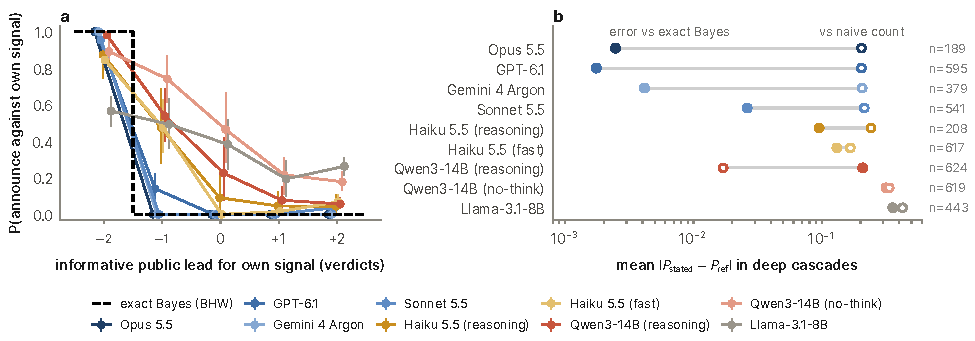
\includegraphics[width=\linewidth]{figs/fig_herding.pdf}
  \caption{\textbf{Frontier agents follow the Bayesian cascade rule and state Bayesian probabilities.}
  (a) Probability of announcing the opposite of one's own spot check, by informative public lead in its
  favour (verdicts protocol). The dashed step is the exact BHW rule; a lead of $-1$ is a Bayes tie. Bins
  with fewer than 10 decisions are omitted. (b) Mean absolute error of the stated $P(\text{compliant})$
  against the exact posterior (filled, ``error vs exact Bayes'') and against a naive count of all verdicts
  (open), over deep-cascade
  positions where the two differ by $\ge 0.10$; log scale. 95\% bootstrap CIs over episodes.}
  \label{fig:herding}
\end{figure}

\begin{figure}[h]
  \centering
  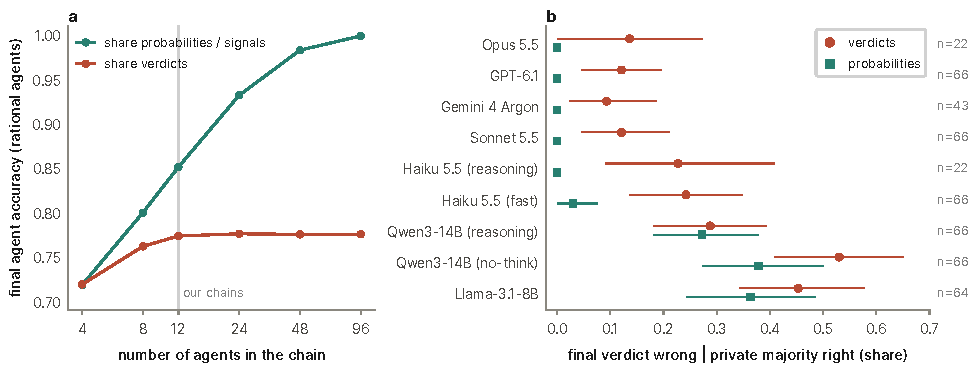
\includegraphics[width=\linewidth]{figs/fig_protocol.pdf}
  \caption{\textbf{Verdict-only protocols cap a rational swarm; sharing probabilities removes the cap.}
  (a) Expected accuracy of the last agent in a chain of perfectly rational agents ($p=0.65$) that share
  verdicts (BHW cascade) or probabilities/signals (full pooling); $2\times10^5$ simulated episodes per point.
  (b) Measured share of episodes whose 12 private spot checks favour the truth but whose final auditor
  announces the wrong answer, under verdicts (circles) and probabilities (squares); 95\% bootstrap CIs;
  $n$ is the number of such episodes.}
  \label{fig:protocol}
\end{figure}

\paragraph{Even honest verdict chains discard information.} Rational chains plateau at 0.775, while pooling
reaches 0.85--0.98 at 12--48 agents; frontier final auditors were wrong in 9--14\% of episodes whose private checks
favoured the truth, and in none with shared probabilities (0 of 22--66; Figure~\ref{fig:protocol}).


\begin{table}[h]
\centering
\scriptsize
\setlength{\tabcolsep}{3.5pt}
\caption{\textbf{Cascade task, all model-modes.} Complete 12-agent chains; override rates when the
informative lead against one's signal is $\ge 2$ (casc.) or $|d|\le1$ excluding ties (none); solo
signal-following; mean $|P-P_B|$ under verdicts; share of deep-cascade positions where $P$ is closer to Bayes
than to the naive count; mean accuracy of agents 3--12 under verdicts, probabilities and the rational
benchmark on the same signals; share of episodes with a correct private majority but a wrong final verdict.
Verdicts that contradict an established cascade are off the rational path; later positions are scored against
the BHW reference that treats such verdicts as uninformative. Excluding them raises Sonnet's closer-to-Bayes share
from 97.6\% to 99.2\% (fast Sonnet: 97\% to 100\%) and lowers its $|P-P_B|$ from 0.020 to 0.013.}
\label{tab:herding}
\resizebox{\linewidth}{!}{\begin{tabular}{lrcccccccccc}
\toprule
 & chains & \multicolumn{2}{c}{override} & solo & $|P-P_B|$ & deep & \multicolumn{3}{c}{pos.\ acc.\ 3--12} & \multicolumn{2}{c}{publicly wrong} \\
\cmidrule(lr){3-4}\cmidrule(lr){8-10}\cmidrule(lr){11-12}
model & & casc. & none & follow & verd. & $\to$B & verd. & prob. & Bayes & verd. & prob. \\
\midrule
Opus 5.5 & 30 & 1.00 & 0.00 & 1.00 & 0.002 & 1.00 & 0.69 & 0.79 & 0.69 & 0.14 & 0.00 \\
GPT-6.1 & 90 & 1.00 & 0.00 & 1.00 & 0.004 & 1.00 & 0.74 & 0.78 & 0.75 & 0.12 & 0.00 \\
Gemini 4 Argon & 60 & 1.00 & 0.00 & 1.00 & 0.003 & 1.00 & 0.75 & 0.77 & 0.75 & 0.09 & 0.00 \\
Sonnet 5.5 & 90 & 0.95 & 0.00 & 1.00 & 0.020 & 0.98 & 0.74 & 0.77 & 0.75 & 0.12 & 0.00 \\
Sonnet 5.5 (fast) & 30 & 0.90 & 0.00 & 1.00 & 0.025 & 0.97 & 0.70 & -- & 0.69 & 0.14 & -- \\
GPT-6.1 (minimal) & 30 & 1.00 & 0.00 & 1.00 & 0.005 & 1.00 & 0.69 & -- & 0.69 & 0.14 & -- \\
Haiku 5.5 (reasoning) & 30 & 0.87 & 0.03 & 1.00 & 0.070 & 0.89 & 0.73 & 0.76 & 0.69 & 0.23 & 0.00 \\
Haiku 5.5 (fast) & 90 & 0.84 & 0.01 & 1.00 & 0.087 & 0.57 & 0.65 & 0.76 & 0.75 & 0.24 & 0.03 \\
Qwen3-14B (reasoning) & 90 & 0.98 & 0.16 & 0.88 & 0.132 & 0.04 & 0.67 & 0.65 & 0.75 & 0.29 & 0.27 \\
Qwen3-14B (no-think) & 90 & 0.89 & 0.29 & 0.70 & 0.251 & 0.57 & 0.55 & 0.59 & 0.75 & 0.53 & 0.38 \\
Llama-3.1-8B & 87 & 0.57 & 0.32 & 0.67 & 0.293 & 0.66 & 0.56 & 0.58 & 0.75 & 0.45 & 0.36 \\
\bottomrule
\end{tabular}
}
\end{table}

\begin{table}[h]
\centering
\small
\caption{\textbf{Two sock-puppets hijack a rational swarm under verdicts; spot checks bound the damage.} Mean
accuracy of the ten genuine auditors / accuracy of the last auditor, after two planted predecessors point
to the wrong state; 30 episodes per cell, same signals as the unplanted runs. The benchmark row simulates
agents who take every predecessor at face value. Fast Haiku repeat run: 0.22/0.37, 0.48/0.67, 0.42/0.57, 0.28/0.37.}
\label{tab:planted}
\begin{tabular}{lcccc}
\toprule
shared after two fake agents & verdicts & spot checks & probs (calibrated) & probs (extreme) \\
\midrule
rational benchmark & 0.00 / 0.00 & 0.45 / 0.66 & 0.45 / 0.66 & 0.01 / 0.09 \\
\midrule
Opus 5.5 & 0.00 / 0.00 & -- & -- & -- \\
GPT-6.1 & 0.00 / 0.00 & 0.48 / 0.60 & 0.49 / 0.63 & 0.51 / 0.70 \\
Sonnet 5.5 & 0.11 / 0.17 & 0.49 / 0.63 & 0.44 / 0.60 & 0.51 / 0.73 \\
Haiku 5.5 (reasoning) & 0.27 / 0.50 & 0.48 / 0.67 & -- & -- \\
Haiku 5.5 (fast) & 0.19 / 0.27 & 0.48 / 0.63 & 0.45 / 0.63 & 0.30 / 0.43 \\
Qwen3-14B (no-think) & 0.53 / 0.53 & 0.65 / 0.63 & 0.62 / 0.60 & 0.64 / 0.60 \\
\bottomrule
\end{tabular}

\end{table}

\begin{table}[h]
\centering
\small
\caption{\textbf{For Sonnet the damage broadly follows the theory across fake positions; Haiku resists head plants.}
Mean accuracy of genuine auditors when fake wrong verdicts occupy the given positions of a 12-auditor chain; in
parentheses, rational agents on the same signals and fake positions. One fake already tips about half of the
chains, because a single wrong genuine signal after it starts a cascade. For mid-chain fakes the rational
benchmark treats fakes that arrive after an established cascade as uninformative (17 of 30 episodes), as in
Table~\ref{tab:herding}. ``--'' fewer than 10 complete episodes (Haiku reasoning, mid-chain: 1 of 10 started).}
\label{tab:sweep}
\begin{tabular}{lccc}
\toprule
fake verdicts & Sonnet & Haiku (reasoning) & Haiku (fast) \\
\midrule
one, position 1 & 0.45 (0.45), $n=20$ & 0.49 (0.43), $n=30$ & 0.41 (0.43), $n=30$ \\
two, positions 1--2 & 0.11 (0.00), $n=30$ & 0.27 (0.00), $n=30$ & 0.19 (0.00), $n=30$ \\
three, positions 1--3 & 0.06 (0.00), $n=20$ & 0.30 (0.00), $n=29$ & 0.23 (0.00), $n=30$ \\
two, positions 5--6 & 0.51 (0.54), $n=16$ & -- & 0.62 (0.59), $n=30$ \\
\bottomrule
\end{tabular}

\end{table}

\begin{table}[h]
\centering
\small
\caption{\textbf{Frontier agents side with Bayes wherever it departs from counting; smaller models fail on
peers' verdicts.} F1--F3: share of discriminating items (32 per family) on which the decision matches Bayes
and not the count, and the largest mean $|P-P_B|$ across the three families. F4: share of cascade-verdict
items (48) on which the stated $P$ is closer to Bayes than to the naive count, and the mean errors against
each. 0 refusals; Llama needed 24 parse retries and left $P$ unparsed on 2 items.}
\label{tab:stress}
\setlength{\tabcolsep}{4pt}
\begin{tabular}{lcccccc}
\toprule
 & \multicolumn{3}{c}{decision $=$ Bayes $\ne$ count} & max $|P-P_B|$ & \multicolumn{2}{c}{F4 cascade} \\
\cmidrule(lr){2-4}\cmidrule(lr){6-7}
model & F1 prior & F2 prec. & F3 echo & F1--F3 & closer & err B / count \\
\midrule
Opus 5.5 & 1.00 & 1.00 & 1.00 & 0.002 & 1.00 & 0.000 / 0.284 \\
GPT-6.1 & 1.00 & 1.00 & 1.00 & 0.000 & 1.00 & 0.002 / 0.286 \\
Gemini 4 Argon & 1.00 & 1.00 & 1.00 & 0.000 & 1.00 & 0.000 / 0.284 \\
Sonnet 5.5 & 1.00 & 1.00 & 1.00 & 0.002 & 0.98 & 0.015 / 0.286 \\
Haiku 5.5 (reasoning) & 1.00 & 0.97 & 0.97 & 0.002 & 0.92 & 0.081 / 0.307 \\
Haiku 5.5 (fast) & 1.00 & 1.00 & 1.00 & 0.005 & 0.44 & 0.211 / 0.208 \\
Qwen3-14B (reasoning) & 0.84 & 0.78 & 0.69 & 0.005 & 0.02 & 0.281 / 0.014 \\
Qwen3-14B (no-think) & 0.53 & 0.50 & 0.44 & 0.281 & 0.58 & 0.337 / 0.418 \\
Llama-3.1-8B & 0.44 & 0.62 & 0.47 & 0.401 & 0.68 & 0.354 / 0.455 \\
\bottomrule
\end{tabular}

\end{table}

\section*{LLM Usage Statement}
% TODO(authors): complete
Large language models were the subjects of these experiments. LLM coding agents also helped write the
experiment code, run analyses, search the literature and draft this report. The authors reviewed the
design, checked the numbers against the raw logs, and take responsibility for the content.

\end{document}
